% --------------------------------------------------------------
% This is all preamble stuff that you don't have to worry about.
% Head down to where it says "Start here"
% --------------------------------------------------------------

\documentclass[12pt]{article}

\usepackage[margin=1in]{geometry}
\usepackage{amsmath,amsthm,amssymb}
\usepackage{enumerate}
\usepackage{graphicx}
\usepackage[english]{babel}
\usepackage[utf8x]{inputenc}
\usepackage[T1]{fontenc}
\usepackage{enumitem}
\usepackage{fancyhdr}
\pagestyle{fancy}
\usepackage[table,xcdraw]{xcolor}

\newcommand{\N}{\mathbb{N}}
\newcommand{\Z}{\mathbb{Z}}
\newcommand{\R}{\mathbb{R}}
\newcommand{\Q}{\mathbb{Q}}
\newcommand{\C}{\mathbb{C}}

\newenvironment{theorem}[2][Theorem]{\begin{trivlist}
\item[\hskip \labelsep {\bfseries #1}\hskip \labelsep {\bfseries #2.}]}{\end{trivlist}}
\newenvironment{lemma}[2][Lemma]{\begin{trivlist}
\item[\hskip \labelsep {\bfseries #1}\hskip \labelsep {\bfseries #2.}]}{\end{trivlist}}
\newenvironment{exercise}[2][Exercise]{\begin{trivlist}
\item[\hskip \labelsep {\bfseries #1}\hskip \labelsep {\bfseries #2.}]}{\end{trivlist}}
\newenvironment{problem}[2][Problem]{\begin{trivlist}
\item[\hskip \labelsep {\bfseries #1}\hskip \labelsep {\bfseries #2.}]}{\end{trivlist}}
\newenvironment{question}[2][Question]{\begin{trivlist}
\item[\hskip \labelsep {\bfseries #1}\hskip \labelsep {\bfseries #2.}]}{\end{trivlist}}
\newenvironment{corollary}[2][Corollary]{\begin{trivlist}
\item[\hskip \labelsep {\bfseries #1}\hskip \labelsep {\bfseries #2.}]}{\end{trivlist}}

\lhead{Report 2, November 10, 2022}
\rhead{Nicholas Tee}

\begin{document}
Link to repo = https://github.com/scandum/wolfsort\\

The workload I chose is a benchmark of a sorting algorithm that the owner of the repository had made. The sorting algorithm in mind is called \textbf{wolfsort}, it is a hybrid sorting algorithm that combines properties of radix sort, quicksort and merge sort. The workload runs a benchmark that compares wolfsort to other hybrid sorting algorithms.

\subsection*{Downloading and running the workload}
To download the repository, run the following command
\begin{verbatim}
git clone https://github.com/scandum/wolfsort
\end{verbatim}
After cloning the repository, you can run and compile the benchmark as such:
\begin{verbatim}
cd wolfsort/src
gcc -O3 bench.c
./a.out
\end{verbatim}
To compile it into a RISC-V binary run the following compile line
\begin{verbatim}
riscv64-linux-gnu-gcc -O3 -static bench.c -o bench.rv 
\end{verbatim}
The bash script I used to run the workload is the following code
\begin{verbatim}
ESESC_BIN=${1:-../main/esesc}

export ESESC_ReportFile="part2Report"
export ESESC_BenchName="./wolfsort/src/bench.rv"
export ESESC_DL1_core_bsize=8
if [ -f $ESESC_BIN ]; then
  $ESESC_BIN 
else
  $ESESC_BenchName 
fi
exit 0
\end{verbatim}
\newpage
\subsection*{Initial Results}
The initial run of the benchmark showed an IPC of 0.41, and a total instruction count of 362,993,027 instructions, with a running time of 702 seconds. The full report given by esesc can be seen below


\begin{figure}[h!]
	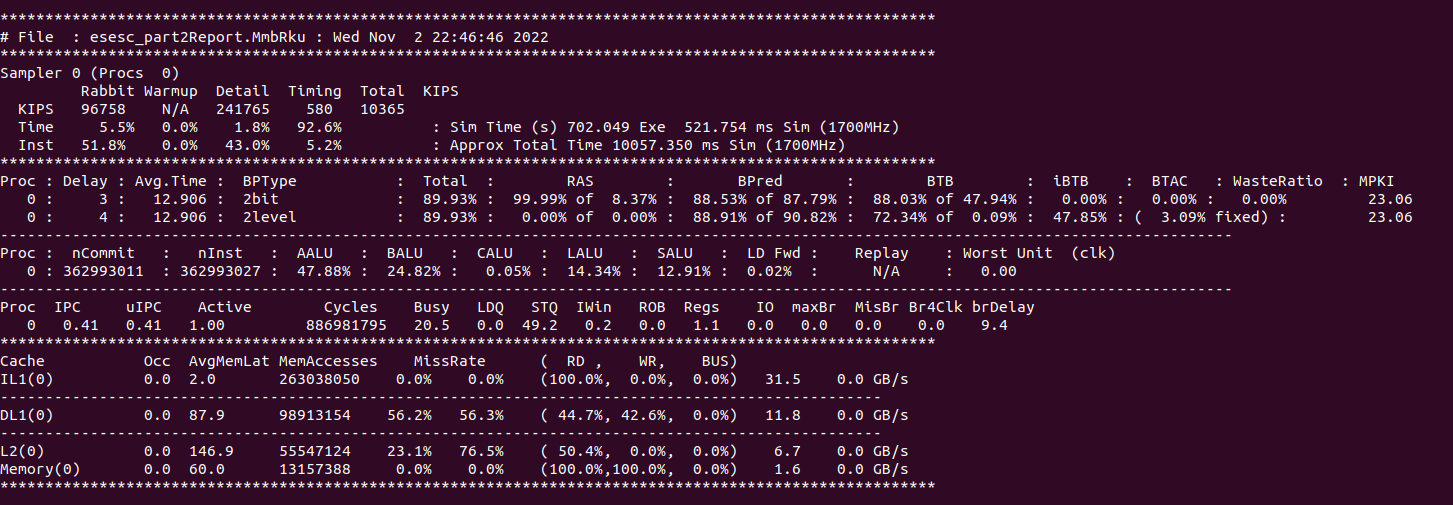
\includegraphics[scale=0.4]{img.png}
\end{figure}

\end{document}